% % % % % % % % % % % % % % % % % % % % % 
% results.tex - Ian Huston
% $Id: results.tex,v 1.25 2009/11/07 13:22:31 ith Exp $
% % % % % % % % % % % % % % % % % % % % % 
% Redefine CVSRevision for this section
\renewcommand{\CVSrevision}{\version$Id: results.tex,v 1.25 2009/11/07 13:22:31 ith Exp $}

% % % % % % % % % % % % % % % % % % % % % % % % % % % % % % % % 
% =========================================================== %
% % % % % % % % % % % % % % % % % % % % % % % % % % % % % % % %
\chapter{Results and Future Work}
\label{ch:results}
% % % % % % % % % % % % % % % % % % % % % % % % % % % % % % % % 
% =========================================================== %
% % % % % % % % % % % % % % % % % % % % % % % % % % % % % % % %


% % % % % % % % % % % % % % % % % % % % % % % % % % % % % % % % 
% =========================================================== %
% % % % % % % % % % % % % % % % % % % % % % % % % % % % % % % %
\section{Introduction}
\label{sec:intro-res}
% % % % % % % % % % % % % % % % % % % % % % % % % % % % % % % % 
% =========================================================== %
% % % % % % % % % % % % % % % % % % % % % % % % % % % % % % % %

The main result of Part~\ref{part:numerical} of this work is the demonstration of a
numerical solution to
the closed Klein-Gordon equation of motion for second order scalar field
perturbations in \eq{eq:KG2-fourier-sr-num}. This includes the slow
roll approximation of the source term for second order perturbations, but the slow
roll version of the evolution equations has not been used for the background or first
order perturbations. In this chapter the results of the numerical calculation
defined in Chapter~\ref{ch:numericalsystem} will be presented. This represents the
first step towards a full calculation of the Klein-Gordon equation at second order.
In addition to the results provided below, plans will be described for future work to
improve the numerical system and increase its applicability. 

As a proof of concept the numerical system was tested with four different
potentials, $V(\vp)=\msqphisq$, $\lambdaphifour$, $\phitwooverthree$ and
$\msqphisqwithV$, and results computed across three
different $k$ ranges. As expected, considering the use of a single slowly
rolling field, the second order perturbation we have calculated is extremely
small in comparison with the first order term. However there are already
differences apparent between the potentials which will be outlined in
Section~\ref{sec:compare-res}.

We have listed the parameters $m$, $\lambda$, $\sigma$ and $m_0$ of the potentials
in Table~\ref{tab:params-num}. These were found using the WMAP5 normalisation
at $\kwmap=0.002 \Mpc^{-1} = 5.25 \e{-60}\Mpl$ \cite{Komatsu:2008hk}.
We have also outlined in \eq{eq:Krangedefns} the three $k$ ranges that have been
used:
% 
\begin{align*}
K_1 &= \left[1.9\e{-5}, 0.039\right]\Mpc^{-1}\,,\quad \Delta k =
3.8\e{-5}\Mpc^{-1} \nonumber\\
K_2 &= \left[5.71\e{-5}, 0.12\right]\Mpc^{-1}\,, \quad \Delta k =
1.2\e{-4}\Mpc^{-1}
\nonumber\\ 
K_3 &= \left[9.52\e{-5}, 0.39\right]\Mpc^{-1}\,, \quad \Delta k =
3.8\e{-4}\Mpc^{-1} \,.
\end{align*}
Many of the results will be quoted for $\kwmap$ which lies in all three of these
ranges.

Given that the first order perturbations for the chosen potentials produce an
almost scale invariant power spectrum with no running, it is no surprise that
the results from the three different $k$ ranges are very similar. The second
order source term is somewhat dependent on the lower bound of $k$ (upper bound
on size). This is expected and in the scale invariant case a log divergence can
be shown to exist \cite{Lyth:2007jh}. We have implemented an arbitrary sharp
cutoff at $\kmin$ below which 
$\dvp1$ is taken to be zero. 
As mentioned in Chapter~\ref{ch:numericalsystem}, there is some evidence to suggest
that a similar cutoff might be supported by the WMAP data
\cite{Sinha:2005mn,Kim:2009pf}. 

In Section~\ref{sec:results} the numerical results for the computation described in
Chapter~\ref{ch:numericalsystem} will be given. Comparisons of the results from the
four different test potentials will be made in Section~\ref{sec:compare-res}. As
this is just the first stage towards a full calculation of the source term the next
steps required will be outlined in Section~\ref{sec:next-res}. Finally in
Section~\ref{sec:disc-num} there will be a discussion of outcomes of the chapter.
% 

% % % % % % % % % % % % % % % % % % % % % % % % % % % % % % % % 
% =========================================================== %
% % % % % % % % % % % % % % % % % % % % % % % % % % % % % % % %
\section{Results}
\label{sec:results}
% % % % % % % % % % % % % % % % % % % % % % % % % % % % % % % % 
% =========================================================== %
% % % % % % % % % % % % % % % % % % % % % % % % % % % % % % % %
In Section~\ref{sec:msqphisq-res} general results will be given demonstrating the
 operation of the numerical system. These results all use the
$V(\vp)=\msqphisq$ potential for the purposes of comparison. The results for the four
different potentials will be compared in Section~\ref{sec:compare-res}.

% % % % % % % % % % % % % % % % % % % % % % % % % % % % % % % % 
% =========================================================== %
% % % % % % % % % % % % % % % % % % % % % % % % % % % % % % % %
\subsection{Results for \texorpdfstring{$V(\vp)=\msqphisq$}{m-squared Model}}
\label{sec:msqphisq-res}
% % % % % % % % % % % % % % % % % % % % % % % % % % % % % % % % 
% =========================================================== %
% % % % % % % % % % % % % % % % % % % % % % % % % % % % % % % %

At first order the solutions obtained agree with previous work in
Refs.~\cite{Salopek:1988qh, Martin:2006rs, Ringeval:2007am}, with oscillations
being damped until horizon crossing (when $k=aH$) after which the
curvature perturbation becomes conserved. Figure~\ref{fig:dp1} shows
the real and imaginary parts of the first order perturbations from
when the initial conditions are set at $k/aH=50$ to just after horizon
crossing. The x-axis for most of the following figures shows the
number of e-foldings left until the end of inflation ($\N_\mathrm{end}-\N$) instead
of the internally used time variable $\N$.
%
% 
\begin{figure}
 \centering
 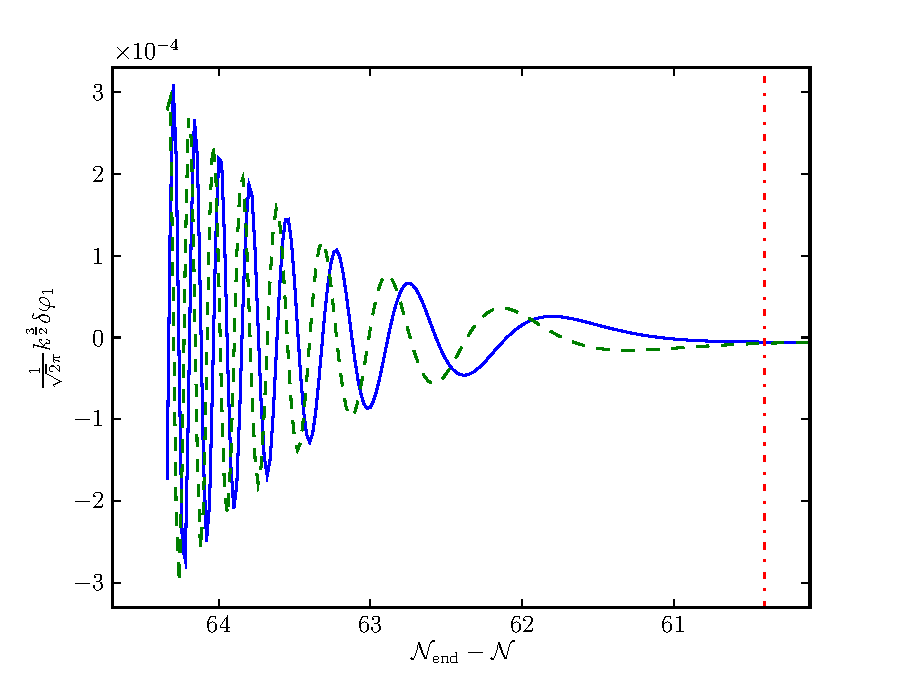
\includegraphics[width=0.8\textwidth]{numerical/graphs/dp1_kwmap}
 \caption[First Order Perturbation]{The first order perturbation $\dvp1$ rescaled by
$k^{3/2}/(\sqrt{2}\pi)$ from the beginning of the simulation until around
horizon crossing (red dot-dashed line). The real (blue) and imaginary (green
dashed) perturbations are shown for $\kwmap$.}
\label{fig:dp1}
\end{figure}
% 
% % % % % % % % % % % % % % % % % % % % % % % % % % % % % % % % % % % 



Figure~\ref{fig:dp2realimag} shows the evolution of the second
order perturbations for $\kwmap$. As mentioned above the
overall amplitude of the second order perturbations is many orders of
magnitude smaller than the first order ones. In Figures~\ref{fig:dp1}
and \ref{fig:dp2realimag} the field values have been rescaled by
$k^{3/2}/(\sqrt{2}\pi)$ to allow a better appreciation of the
magnitude of the resulting power spectra.
% 
\begin{figure}
 \centering
 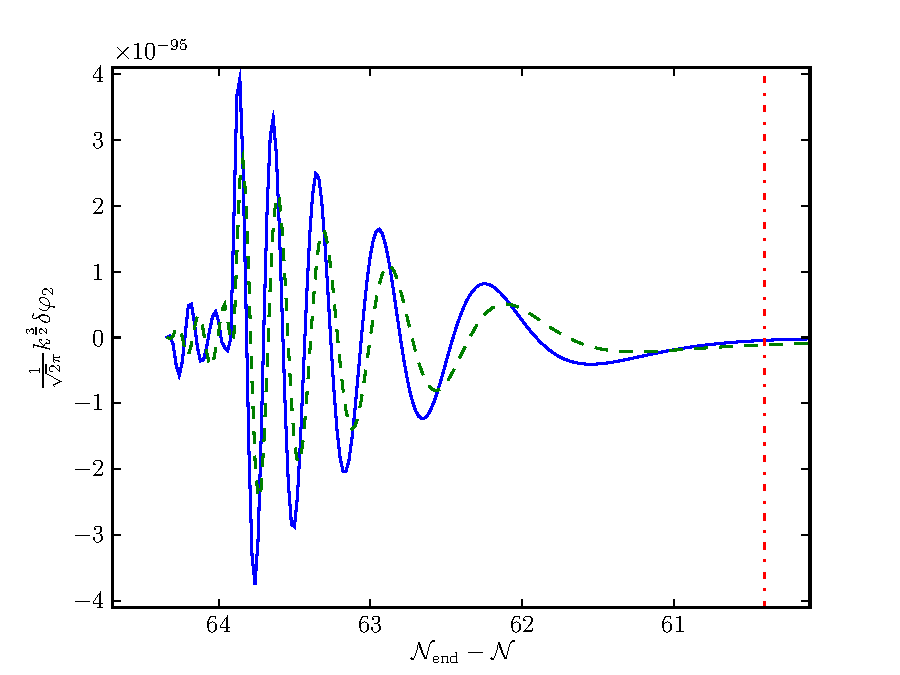
\includegraphics[width=0.8\textwidth]{numerical/graphs/dp2_kwmap}
 \caption[Second Order Perturbation]{The real (blue line) and imaginary (green
dashed) components of the
second order
perturbation $\dvp2(\kwmap)$ from the beginning of the simulation until around
the time
of horizon exit (red dot-dashed line).}
\label{fig:dp2realimag}
\end{figure}
% 
% % % % % % % % % % % % % % % % % % % % % % % % % % % % % % % % % % % 



The source term $S(\kvi)$ is calculated using \eq{eq:KG2-src-sr-aterms} at each time
step using the results of the first order and background runs. This term
drives the production of second order perturbations as shown in
\eqs{eq:KG2-fourier-sr-num} and
\eqref{eq:KG2-fourier-sr-ntime}. Figure~\ref{fig:src-full} shows the
absolute magnitude of the source term for a single $k$ mode, $\kwmap$,
for all time steps calculated.
% 
\begin{figure}
\centering
\subfloat[Absolute magnitude of the source term.]{
 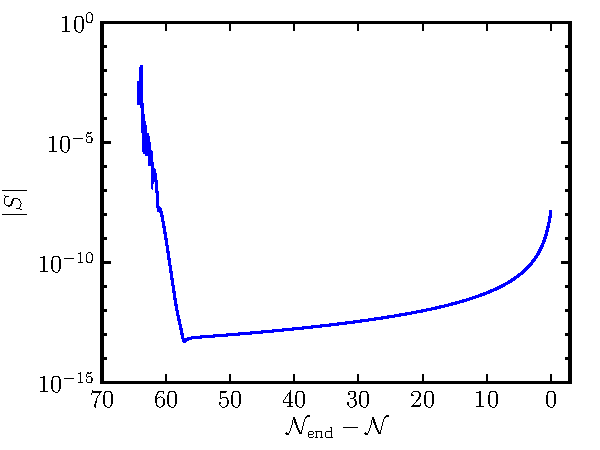
\includegraphics[width=0.43\textwidth]{numerical/graphs/src-kwmap-small}
\label{fig:src-full}
}\qquad
% 
\subfloat[Power spectrum of scalar perturbations][Power spectrum of scalar
perturbations $\mathcal{P}^2_{\delta\varphi} =
\frac{k^3}{2\pi^2}|\delta\varphi|^2$.]{
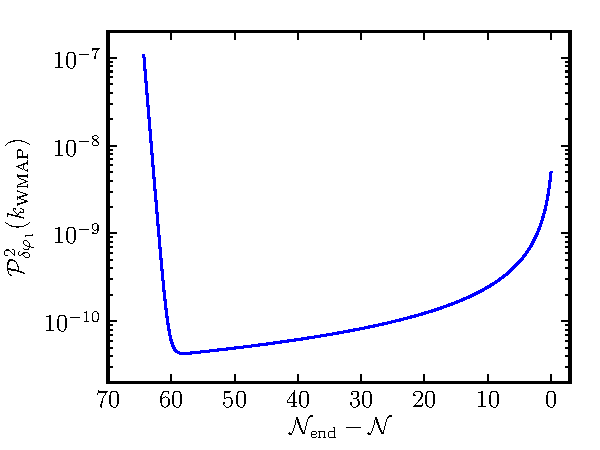
\includegraphics[width=0.43\textwidth]{numerical/graphs/Pphi-kwmap-nohoriz-small}
\label{fig:Pphi-kwmap}
}
\caption[The source term and power spectrum for $\kwmap$]{Source term and power
spectrum for the WMAP pivot scale $\kwmap$.}
\end{figure}
% 
Figure~\ref{fig:src-kwmap-3ranges} shows how the source term changes
with the choice of $k$ range.  After horizon crossing the source terms
are approximately equal. Before horizon crossing, however, there is a
strict hierarchy with the smaller $k$ ranges, $K_1$ and $K_2$, leading to
smaller source
contributions.  As stated in Section \ref{sec:tests-num}, $\Delta k$
should be at least as large as $\kmin$ in order to reduce the error to
a minimum.
% 
\begin{figure}
\centering
 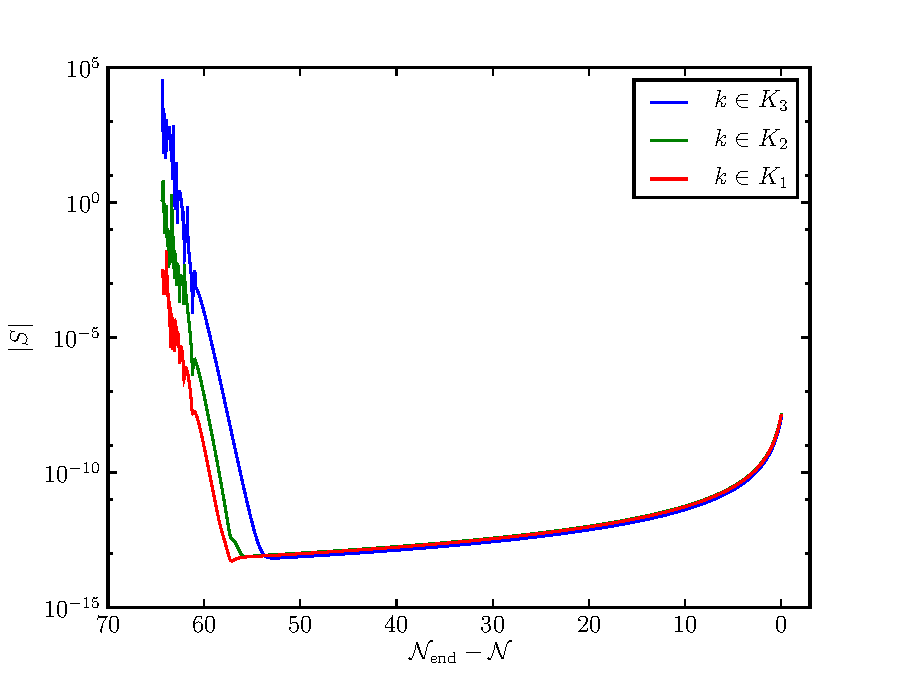
\includegraphics[width=0.8\textwidth]{numerical/graphs/src-kwmap-3ranges-large}
\caption[Comparison of source term for different ranges]{Comparison of the source
term \eqref{eq:KG2-source-ntime} for $\kwmap$ over three different ranges with
different $\Delta k$s as specified
in
\eq{eq:Krangedefns}.} 
\label{fig:src-kwmap-3ranges}
\end{figure}
% 
\begin{figure}
\centering
 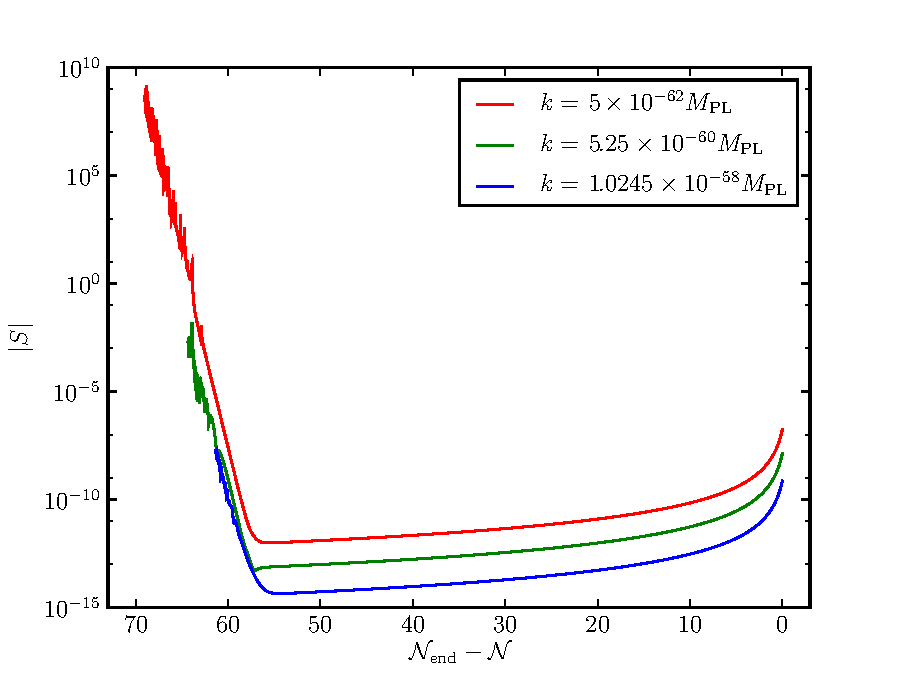
\includegraphics[width=0.8\textwidth]{numerical/graphs/src-3ks-large}
\caption[Source term at three different $k$s]{The source term
\eqref{eq:KG2-source-ntime} for three different $k$
values including the WMAP
pivot scale. As $k$
gets larger (scale gets smaller) the source term becomes smaller.}
\label{fig:src-3ks}
\end{figure}
% 
% 



The source term is large at early times, and closely follows the form
of the spectrum of the first order perturbations as can be seen from
Figure~\ref{fig:Pphi-kwmap}.
%
It is informative to compare the magnitude of the source term with the
other terms in the second order evolution equation
(\ref{eq:KG2-fourier-sr-ntime}). If we let $T$ denote the other terms,
%
\begin{equation}
\label{eq:Tdefn}
 T(\kvi) = \left(3 + \frac{\dN{H}}{H}\right)
\dN{\dvp2}(\kvi)+ \left(\frac{k}{aH}\right)^2\dvp2(\kvi)
+\left(\frac{\Upp}{H^2}-{24 \pi G}(\dN{\vp_{0}})^2\right)
\dvp2(\kvi) \,,
\end{equation}
%
then Figure~\ref{fig:src-vs-others} shows the absolute magnitude of
both $S$ and $T$.  It is clear that for this $k$ the source term is of comparable
magnitude only early in the simulation.  Figure~\ref{fig:s-over-t-3ks}
shows a comparison of $|S|/|T|$ for three different $k$ values. The larger the
$k$ mode, the closer in amplitude $S$ is to the rest of the terms in the ODE.
A priori it is not known where $S$ will be large for a particular chosen potential
and mode but once determined it could be possible to significantly reduce the time
required for the simulation by only calculating $S$ in the regions where it is
important.
%
\begin{figure}
\centering
 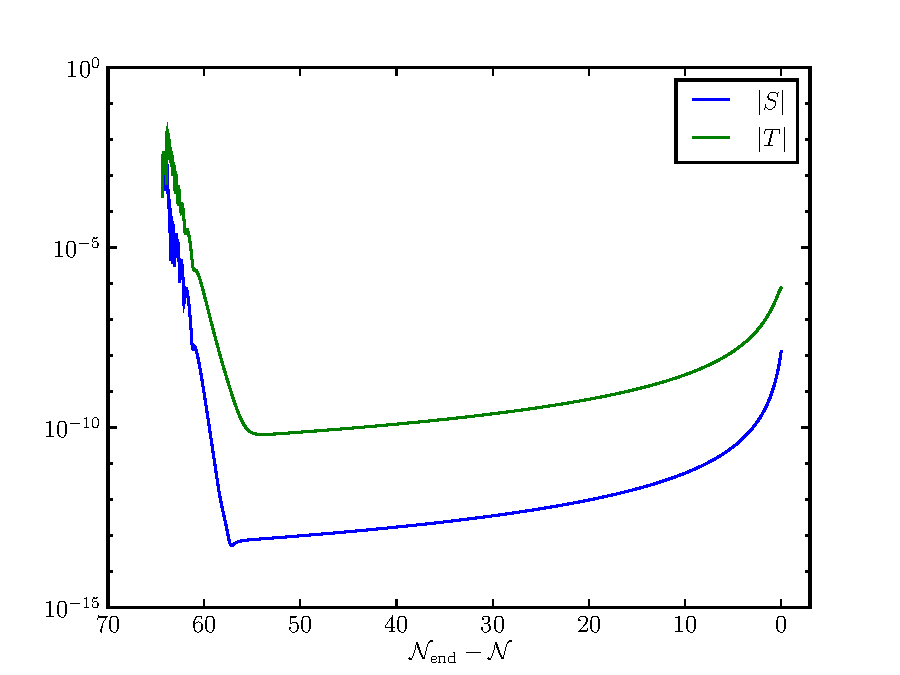
\includegraphics[width=0.8\textwidth]{numerical/graphs/src-vs-t-kwmap-large}
\caption[Source term compared to $T$ term]{The source term (lower blue line), as
defined in \eq{eq:KG2-source-ntime}, is
compared with the $T$ term
(upper green line), as defined in \eq{eq:Tdefn}, for $\kwmap$. The source term is of
comparable magnitude at the beginning of the simulation.}
 \label{fig:src-vs-others}
\end{figure}
% 

\begin{figure}
\centering
 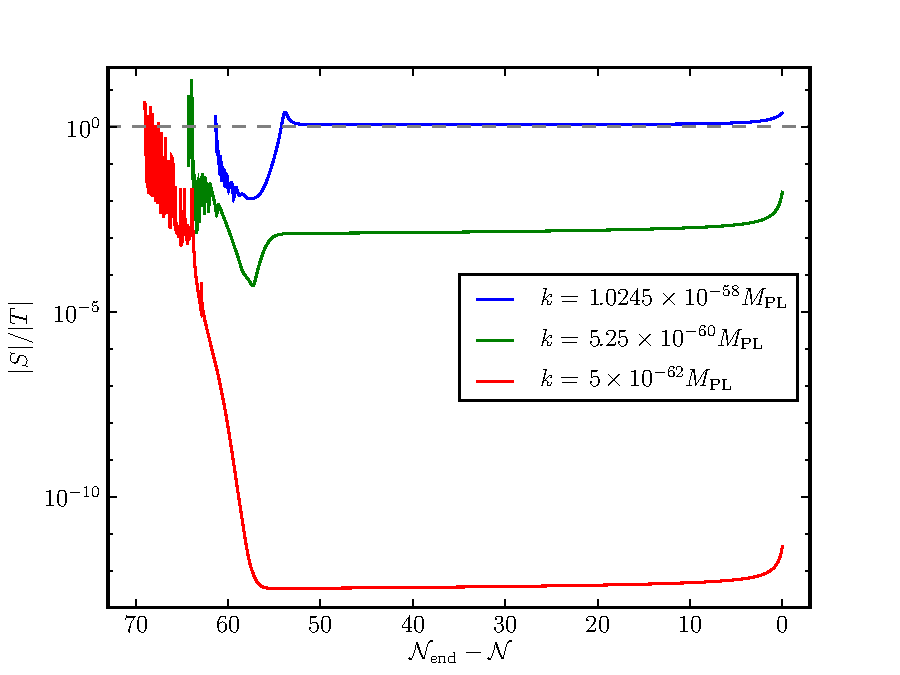
\includegraphics[width=0.8\textwidth]{numerical/graphs/s-over-t-3ks-large}
\caption[Quotient of $S$ and $T$]{The quotient of the $S$ term,
\eq{eq:KG2-source-ntime}, and the $T$ term, \eq{eq:Tdefn}, for three
different $k$ values
including the WMAP pivot scale. Depending on $k$ the source term only dominates
at early stages or is important throughout the evolution.}
 \label{fig:s-over-t-3ks}
\end{figure}
% 
% 

% % % % % % % % % % % % % % % % % % % % % % % % % % % % % % % % % % %

In Figure~\ref{fig:src-kinit} the value of $|S|$ at the start of the evolution
of $\dvp2$ for each $k$ mode is shown. The magnitude of the source term is much
smaller for larger $k$s (smaller scales). 
Because the smaller $k$s begin their evolution earlier the relative difference
in $|S|$ is not as pronounced when measured at a single timestep (see for example
Figure~\ref{fig:src-3ks}).
It should also be remembered that the magnitude of other terms in the second
order ODE is small for larger $k$s as shown by the ratio $|S|/|T|$ in
Figure~\ref{fig:s-over-t-3ks} where $T$ is defined above in \eq{eq:Tdefn}.
% 
\begin{figure}
\centering
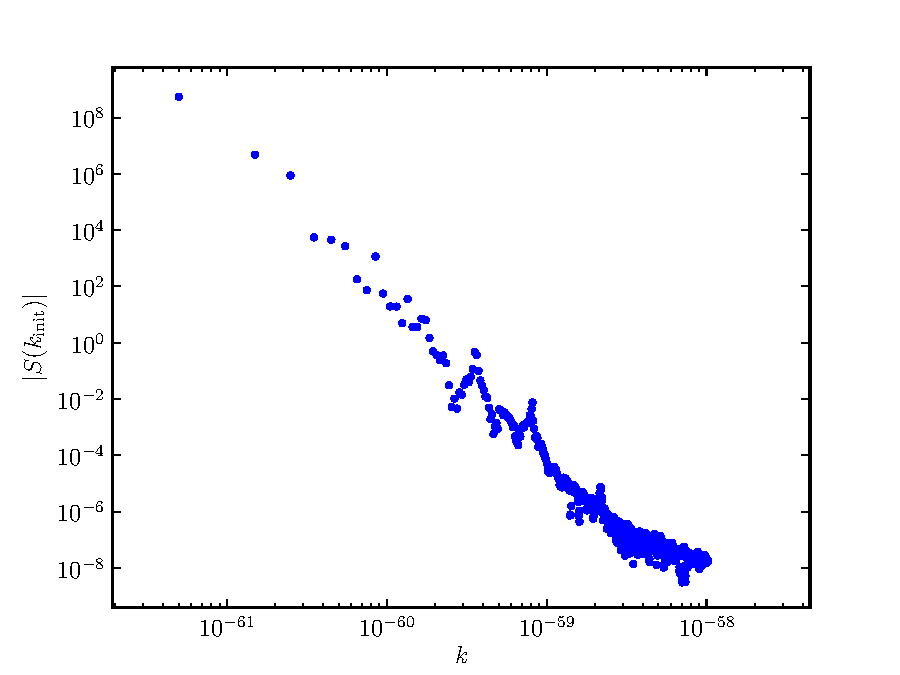
\includegraphics[width=0.8\textwidth]{numerical/graphs/src_kinit_log}
 \caption[Source term at initial start times]{The absolute magnitude of the source 
term at the initial start time for each $k$ when $k = aH \times 50$ deep inside the
horizon. The results are for the range $K_1=\left[ 1.9\e{-5},
0.039 \right] \Mpc^{-1}= \left[0.5\e{-61}, 1.0245\e{-58}\right]\Mpl$.}
\label{fig:src-kinit}
\end{figure}
% 

The source term for all $k$s can also be compared for different timesteps. In
Figure~\ref{fig:src-3ns} the upper blue line shows $|S(k)|$ around 69 e-foldings
before the end of
inflation when $\dvp1$ has been initialised for only the very smallest $k$
modes. The middle green
line shows $|S|$ when all $\dvp1$ modes have been started. Finally the lower red
line plots $|S|$
after all modes have exited the horizon, around 52 e-foldings before the end of
inflation.
% 
\begin{figure}
\centering
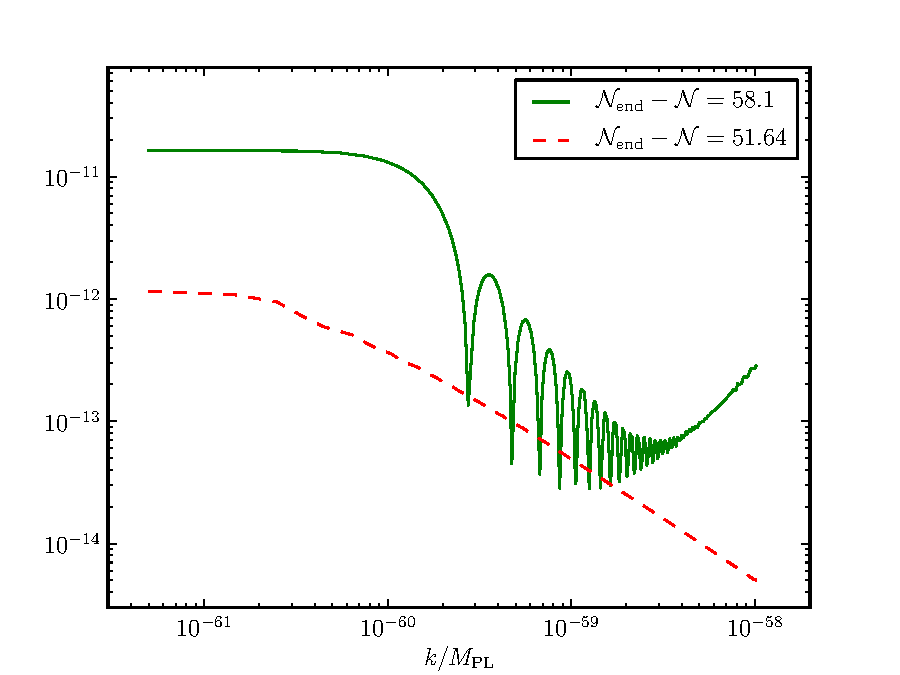
\includegraphics[width=0.8\textwidth]{numerical/graphs/src_3ns-large}
\caption[Source term at three different times]{The absolute magnitude of the source 
term for all $ks$ in the range at three different timesteps: the upper blue line when
only the largest modes have been initialised; the middle green line when all modes
have been initialised; and the lower red dashed line when all modes have
exited the horizon. The $k$ range shown here is $K_1=\left[ 1.9\e{-5}, 0.039
\right] \Mpc^{-1}= \left[0.5\e{-61}, 1.0245\e{-58}\right]\Mpl$.}
\label{fig:src-3ns}
\end{figure}
% 
% % % % % % % % % % % % % % % % % % % % % % % % % % % % % % % % 




% % % % % % % % % % % % % % % % % % % % % % % % % % % % % % % % 
% =========================================================== %
% % % % % % % % % % % % % % % % % % % % % % % % % % % % % % % %
\subsection{Comparison of Models}
\label{sec:compare-res}
% % % % % % % % % % % % % % % % % % % % % % % % % % % % % % % % 
% =========================================================== %
% % % % % % % % % % % % % % % % % % % % % % % % % % % % % % % %
All the results quoted so far are for the $V(\vp)=\msqphisq$ model. In this section
the results for all four potentials will be compared using the $K_2$ range for $k$. 
% 
% 
\begin{figure}
 \centering
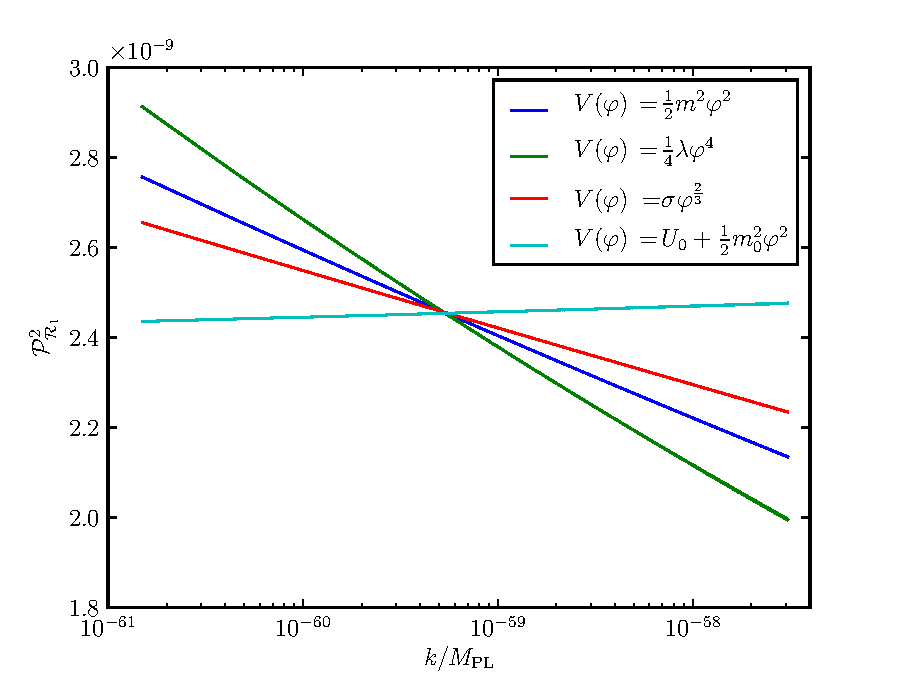
\includegraphics[width=0.8\textwidth]{numerical/graphs/cmp_Pr_allks-large}
\caption[Comparison of $\Pr$ for models]{Comparison of the power spectrum $\Pr$ for
the four different models. The three models $V(\vp)=\msqphisq$, $\lambdaphifour$ and
$\phitwooverthree$ have red spectra ($n_s <1$) while the $V(\vp) = \msqphisqwithV$
model has a blue spectrum ($n_s>1$).}
\label{fig:cmp-Pr}
\end{figure}
% 
Figure~\ref{fig:cmp-Pr} shows the power spectrum of curvature perturbations, $\Pr$, for each
potential. The $\msqphisq$, $\lambdaphifour$ and $\phitwooverthree$ models all
clearly have
a red spectrum with $n_s <1$. On the other hand the $\msqphisqwithV$ model has
a blue
spectrum ($n_s>1$) when $U_0$ to chosen to be $5\e{-10}\Mpl^4$ as specified in
Section~\ref{sec:pots-num}. 
% 
The values of $n_s$ obtained for the four potentials are given in Table~\ref{table:ns-res}. 
% 
\begin{table}
\begin{center}
% use packages: array
\begin{tabular}{ccr}
\toprule
Potential & $n_s$ & $n_s - 1$ \\
\midrule
$\msqphisq$ & 0.965 & -0.035 \\ 
% \hline
$\lambdaphifour$ & 0.949 & -0.051 \\
% \hline 
$\phitwooverthree$ & 0.977 & -0.023 \\
% \hline 
$\msqphisqwithV$ & 1.002 & 0.002 \\
\bottomrule
\end{tabular}
\caption{Spectral index values for the four potentials.}
\label{table:ns-res}
\end{center}
\end{table}


\begin{figure}[h]
\centering%
\subfloat[$V(\vp)=\msqphisq$]{
 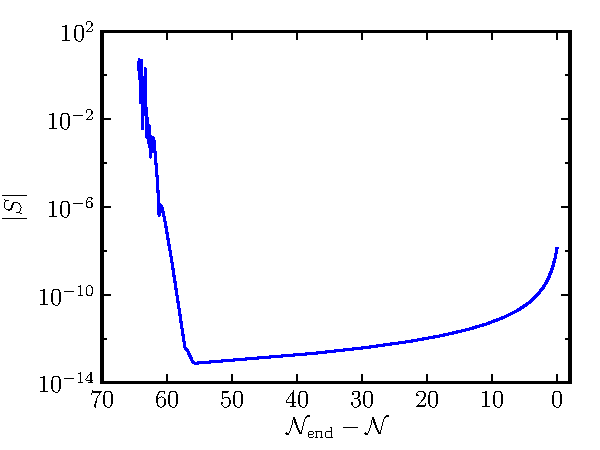
\includegraphics[width=0.43\textwidth]{numerical/graphs/src_onek_msqphisq-small}
}\qquad%
\subfloat[$V(\vp)=\lambdaphifour$]{
 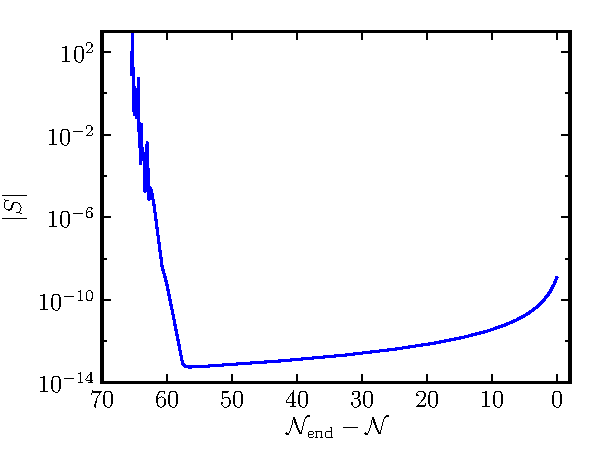
\includegraphics[width=0.43\textwidth]{numerical/graphs/src_onek_lambdaphi4-small}
}\\%
\subfloat[$V(\vp)=\phitwooverthree$]{
 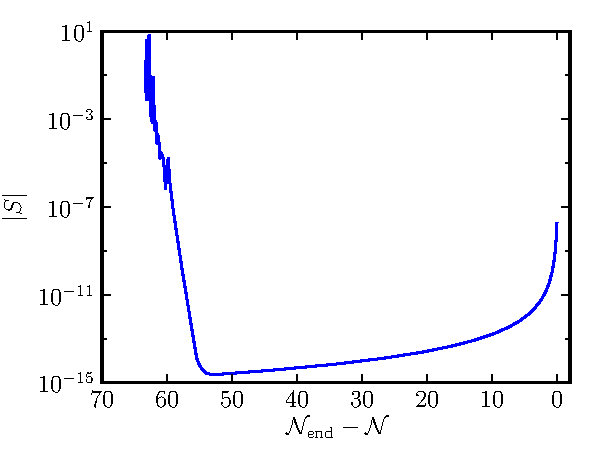
\includegraphics[width=0.43\textwidth]{numerical/graphs/src_onek_phi2over3-small}
}\qquad%
\subfloat[$V(\vp)=\msqphisqwithV$]{
 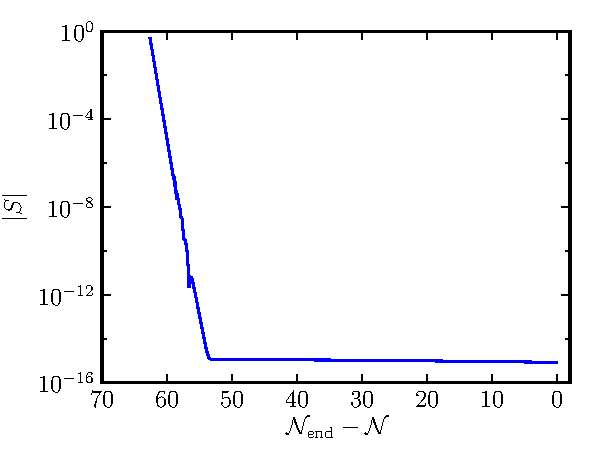
\includegraphics[width=0.43\textwidth]
  {numerical/graphs/src_onek_msqphisq_withV0-small}
}
\caption[The source term for different potentials]{Plots of the source term for the
four different potentials used.}
\label{fig:sourcecomparison-res}
\end{figure}
% 
The source term for each model is shown separately in Figure~\ref{fig:sourcecomparison-res} for
$\kwmap$ using the $K_2$ range\footnotemark. 
% 
\footnotetext{These plots use a different $k$ range to the ones comparing $V(\vp)=\msqphisq$ and
$\lambdaphifour$ in \Rref{hustonmalik}.}
% 
While clearly these source terms are superficially similar
there are differences apparent. In Figure~\ref{fig:cmp-src-kwmap} the source terms are plotted
together for $\kwmap$. The $\kwmap$ mode begins at different times for the
different models. To enable comparison each result is plotted in terms of the
initialisation time for that mode.  The change in duration is a consequence of
allowing $H$ to evolve during the calculation. 

\begin{figure}
 \centering
 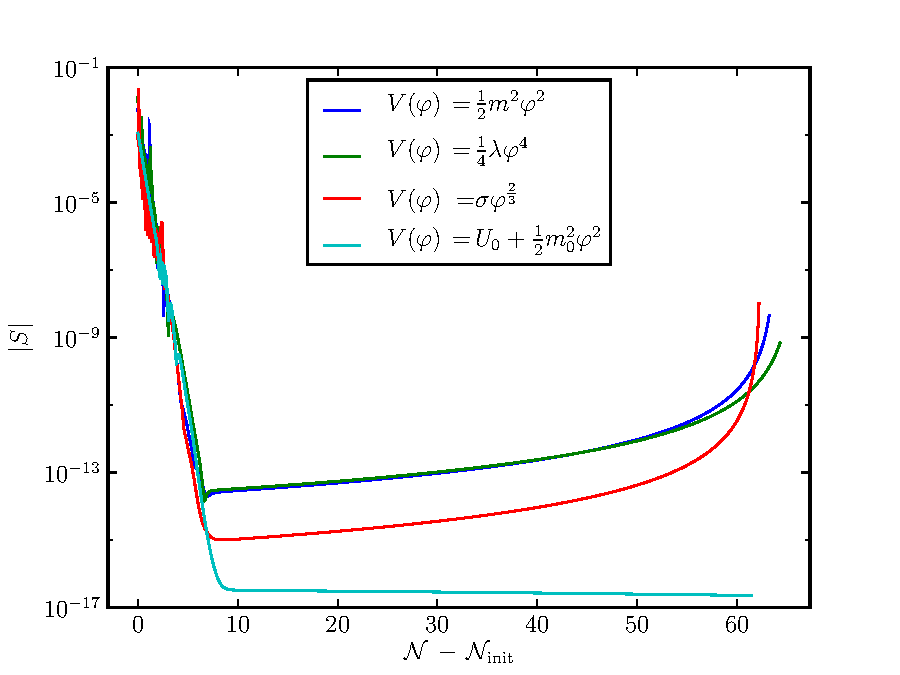
\includegraphics[width=0.8\textwidth]{numerical/graphs/cmp_src_kwmap-large}
 \caption[Comparison of source term for models]{Comparison of the source term
evolution for the four different models.}
\label{fig:cmp-src-kwmap}
\end{figure}
% 

The source term results for the $V(\vp)=\msqphisq$ and $\lambdaphifour$ models are very similar.
From horizon crossing to near the end of inflation the results appear to coincide.
The $\lambdaphifour$ mode has a slightly longer duration and at late times is reduced in comparison
with the $\msqphisq$ one. Figure~\ref{fig:cmp-src-zoom-kwmap} shows that at early times the
relationship is more complicated with the $\lambdaphifour$ mode being larger for a significant
period.

In the early stages the amplitude of the $V(\vp)=\phitwooverthree$ model is very
similar to the other two
results described above. After horizon crossing however there is a significant drop in the
amplitude of $S$ in comparison with the $\msqphisq$ and $\lambdaphifour$ models. This
continues
until late in the evolution when $|S|$ increases swiftly to reach levels above the
others.
The duration of the mode in this model is shorter than in the other two models
described so far. 

\begin{figure}
 \centering
 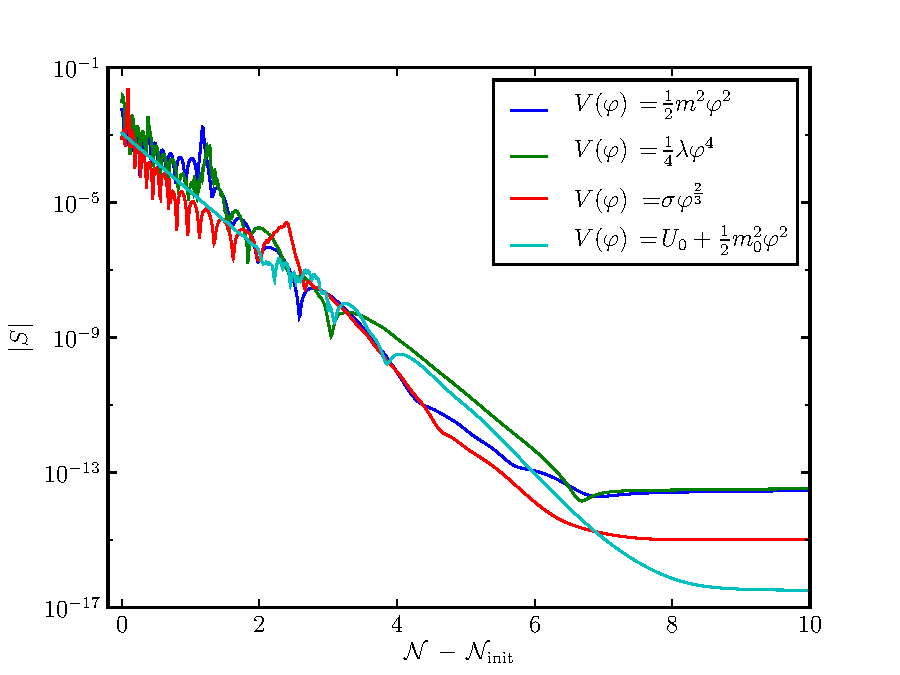
\includegraphics[width=0.8\textwidth]{numerical/graphs/cmp_src_kwmap_zoom-large}
 \caption[Comparison of source term for models at early stage]{Comparison of the
source term evolution for the four different models at early times.}
\label{fig:cmp-src-zoom-kwmap}
\end{figure}
% 

The final model, $V(\vp)=\msqphisqwithV$, is nominally a hybrid inflation model
requiring two fields.
As described in Section~\ref{sec:pots-num}, in order to evaluate using the single field
calculation, the end time of inflation must be specified by hand. In this simulation
$\vp\simeq 8$
is taken as the end time. In this region the potential is extremely flat and the effect of this can
be seen in the source term of the model. Before horizon crossing it is of comparable magnitude to
the other terms. However a steep descent ensures that it is a few orders of magnitude
smaller than
the other terms after horizon crossing. In contrast to the behaviour of the other models, the source
term does not increase close to the end of inflation. This is due to the enforced end time cut-off
which means that $\bar{\varepsilon}_H$ does not become large.

In this section we have described the results for four different single field potentials. As
expected for single field slow roll models they exhibit similar properties. In the next section
plans to extend the calculation to deal with more interesting models will be outlined.

% % % % % % % % % % % % % % % % % % % % % % % % % % % % % % % % 
% =========================================================== %
% % % % % % % % % % % % % % % % % % % % % % % % % % % % % % % %
\section{Next Steps}
\label{sec:next-res}
% % % % % % % % % % % % % % % % % % % % % % % % % % % % % % % % 
% =========================================================== %
% % % % % % % % % % % % % % % % % % % % % % % % % % % % % % % %

There are many possible next steps to improve the program outlined in
Chapter \ref{ch:numericalsystem}. Chief amongst these is the implementation of the
full second order source term given in \eqs{eq:SOKG-real-num} and
\eqref{eq:Fdvk1-fourier-num}. Although clearly
more complicated than the slow roll case in \eq{eq:KG2-fourier-sr-ntime},
only three more $\theta$ dependent terms need to be added to the $\A$--$\D$ terms
listed in \eq{eq:AtoD-num}.  The four potentials used above are all slowly rolling
during inflation. Therefore it is not expected that
using the full source equation would result in an appreciably
different outcome in these models until near the end of the inflationary phase. Once
the field has stopped rolling slowly, new observable features might
arise as is indeed the case at first order. 


To set up the numerical system to use the full second order equation
\eqs{eq:SOKG-real-num} and \eqref{eq:Fdvk1-fourier-num}, they must be written in
terms of $\N$ with the $\theta$ dependent terms grouped together. The main equation
becomes
\begin{multline}
 \label{eq:fullso-res}
\ddN{\dvp2} + \left(3 + \frac{\dN{H}}{H}\right) \dN{\dvp2} +
\left(\frac{k}{aH}\right)^2 \dvp2 \\
% 
+ \frac{1}{H^2}\left[ \Upp + 8\pi G\left(2\dN{\vp_0}\Uphi + 8\pi G
\left(\dN{\vp_0}\right)^2 \U \right)\right] 
% 
+ S_\mathrm{full}(\kvi) = 0\,,
\end{multline}
% 
and the full source equation is given by
% 
\begin{align}
\label{eq:fullsrc-res}
S_\mathrm{full}(\kvi) = \frac{1}{(2\pi)^2}\int \d q q^2 &\Bigg\{ 
% 
\frac{1}{\left(H\right)^2} \left[ \Uppp + 3(8\pi G)\dN{\vp_0}\Upp\right]
 \dvp1(\qvi) \A(\kvi, \qvi) \nonumber \\
% 
&+\frac{(8\pi G)^2 \dN{\vp_0}}{(aH)^2}\left[ 2a^2\dN{\vp_0}\Uphi +\dN{\vp_0}Q
-\frac{Q^2}{2(aH)^2}\right] \dvp1(\qvi) \A(\kvi, \qvi) \nonumber \\
% 
&- \frac{(8\pi G)^2}{(aH)^2}\frac{(\dN{\vp_0})^2 Q}{2} \dN{\dvp1}(\qvi)
\A(\kvi, \qvi) \nonumber \\
% 
&+ \frac{2(8\pi G)Q}{(aH)^2} \dvp1(\qvi)\wt{\C}(\kvi, \qvi) 
% 
+ \frac{8\pi G \dN{\vp_0}}{2} \dN{\dvp1}(\qvi) \wt{\C}(\kvi, \qvi) \Bigg\} \nonumber
\\
% 
&+ F_\mathrm{full}(\dvp1(\kvi), \dN{\dvp1}(\kvi))\,.
\end{align}
% 
The $F_\mathrm{full}$ term in \eq{eq:fullsrc-res} requires the use of three further
$\theta$
integrals in addition to those in \eq{eq:AtoD-num}:
% 
\begin{align}
\label{eq:efg-terms-res}
 \E(\kvi, \qvi) &= \int_0^\pi \cos^3(\theta) \sin(\theta) \dvp1(\kvi-\qvi)\d \theta
\,,\nonumber \\
% 
\F(\kvi, \qvi) &= \int_0^\pi \frac{\sin^3(\theta)}{|\kvi-\qvi|^2} \dvp1(\kvi-\qvi)\d
\theta \,,\nonumber \\
% 
\wt{\G}(\kvi, \qvi) &= \int_0^\pi \frac{\sin^3(\theta)}{|\kvi-\qvi|^2}
\dN{\dvp1}(\kvi-\qvi)\d \theta \,.
\end{align}
% 
It is worth noting that the term $\sin^3(\theta)/|\kvi-\qvi|^2$ goes to $0$ in the
limit when $k=q$ and
$\theta\rightarrow 0$.
% 
Using the terms $\E$, $\F$ and $\wt{\G}$, the $F_\mathrm{full}$ term can now be
written:
\begin{align}
 \label{eq:fullfterm-res}
F_\mathrm{full} &= \frac{8\pi G}{(2\pi)^2}\frac{1}{(aH)^2} \int \d q\, q^2 \Bigg\{
\nonumber \\
% 
&  \dN{\vp_0}\Bigg[ \left(2k^2 + \left(\frac{7}{2} - \frac{8\pi
G}{4}(\dN{\vp_0})^2 \right)q^2 + \frac{3}{4}\frac{8\pi G}{(aH)^2} X^2 \right)
\dvp1(\qvi) \nonumber \\
% 
& \qquad + (8\pi G) Q \dN{\vp_0} \left(\frac{3}{4} + \frac{q^2}{k^2}\right)
 \dN{\dvp1}(\qvi) \Bigg] \A(\kvi, \qvi) \nonumber \\
% 
&+ \Bigg[ \left( 2Q \frac{q}{k} \left(1- \frac{8\pi G}{(aH)^2} Q \dN{\vp_0}\right)
-\frac{9}{2} \dN{\vp_0} k q - \dN{\vp_0} \frac{q^3}{k}\right) \dvp1(\qvi) \nonumber
\\
% 
&\qquad - 2Q (8\pi G) (\dN{\vp_0})^2\frac{q}{k} \dN{\dvp1}(\qvi)\Bigg] \B(\kvi, \qvi)
\nonumber \displaybreak[0]\\
% 
&+ \Bigg[ \left(-2 + (8\pi G)(\dN{\vp_0})^2 \left(\frac{1}{4} + \frac{1}{2aH}\right)
\right) Q \dvp1(\qvi) \nonumber \\
% 
&\qquad + \left(\frac{8\pi G}{4}(\dN{\vp_0})^2 -2\right) \dN{\vp_0} (aH)^2
\dN{\dvp1}(\qvi)\Bigg] \wt{\C}(\kvi, \qvi)\nonumber \\
% 
&+ \Bigg[ 2Q \frac{k}{q}\dvp1(\qvi) + \left(2\frac{k}{q}-\frac{q}{k}\right)
\dN{\vp_0} (aH)^2 \dN{\dvp1}(\qvi) \Bigg]\wt{\D}(\kvi, \qvi) \nonumber \\
% 
&+ (8\pi G) \dN{\vp_0} \Bigg[ \left(\frac{1}{4}(\dN{\vp_0})^2q^2 +
\frac{Q^2}{2(aH)^2}\right) \dvp1(\qvi) + \frac{Q}{2}\dN{\vp_0} \dN{\dvp1}(\qvi)
\Bigg] \E(\kvi, \qvi) \nonumber \displaybreak[0]\\
% 
&+ (8\pi G)^2 \dN{\vp_0} Q \Bigg[ -\frac{Q}{2(aH)^2}\left(\frac{k^2}{2}+q^2\right)
\dvp1(\qvi) - \frac{1}{4} \dN{\vp_0} k^2 \dN{\dvp1}(\qvi) \Bigg] \F(\kvi, \qvi)
\nonumber \\
% 
&+ (8\pi G)^2 (\dN{\vp_0})^2 \Bigg[ -\frac{Q}{2}\left(\frac{k^2}{2} +
\frac{q^2}{aH}\right)\dvp1(\qvi) -\frac{(aH)^2}{4}\dN{\vp_0}k^2 \dN{\dvp1}(\qvi)
\Bigg] \wt{\G}(\kvi, \qvi) \Bigg\} \,.
\end{align}
% 
This set of equations is clearly much longer than the slow roll ones used in
Chapter~\ref{ch:numericalsystem}. The numerical complexity is, however, not
much greater, once the three terms in \eq{eq:efg-terms-res} are calculated. The
running
time of the full calculation will clearly be a significant constraint.

With this in mind, the performance of the numerical simulation could be improved by
analysing the most time consuming processes and investigating what
optimisations could be implemented. The realisation of the current, perhaps
inelegant, procedure will allow any performance improvements to be benchmarked for
accuracy as well as speed.
% 
As discussed above $N_k$ was set to $1025$ for the test runs. This provides good
coverage of the
WMAP $k$ range but it is not clear whether it sufficiently
approximates the integral to infinity for the source term.  Currently
logistical factors, including the running time and memory usage of the code,
restrict the choice of $N_k$. By optimising the routines
for reduced memory and increased speed it should be possible to extend the $k$ ranges
and increase the resolution. 


Beyond these considerations the next step is to implement a multi-field
version of the system. This would allow the investigation of models that inherently
produce large second order perturbations. In \Rref{Malik:2006ir} the
second order Klein-Gordon equation is given for multiple fields and upgrading the
simulation to use these equations should be a straight-forward, if lengthy, process.
Extending the current data-structures and routines to a fixed number of extra fields
will increase the numerical complexity and the run-time of the code. 



% 
% 
% 
% % % % % % % % % % % % % % % % % % % % % % % % % % % % % % % % 
% =========================================================== %
% % % % % % % % % % % % % % % % % % % % % % % % % % % % % % % %
\section{Discussion}
\label{sec:disc-num}
% % % % % % % % % % % % % % % % % % % % % % % % % % % % % % % % 
% =========================================================== %
% % % % % % % % % % % % % % % % % % % % % % % % % % % % % % % %

Part~\ref{part:numerical} of this work described the numerical
solution of the evolution equations for second order scalar perturbations, using the
closed form of the Klein-Gordon equation in \eq{eq:KG2-fourier-sr-num}. Direct
calculation of field perturbations beyond
first order using perturbation theory has been shown to be readily achievable, though
not trivial.

This first demonstration has been limited to considering
the slow roll approximation of the source term in \eq{eq:KG2-fourier-sr-num} which
is quadratic in first order perturbations. Slow roll has not been imposed on the
background or first order equations. Four different
potentials
$V(\vp)=\msqphisq$, $\lambdaphifour$, $\phitwooverthree$ and $\msqphisqwithV$ were
used to demonstrate the capabilities of the
system. The singularity at $k=0$ which arises as larger and larger
scales are considered is avoided by implementing a cutoff at small
wavenumbers below $\kmin$. This is a pragmatic choice necessary for
the calculation.
It is also necessary to
pick a maximum $k$ value, and this choice is dictated by computational
resources and with reference to observationally relevant scales. In
this demonstration $k$ ranges have been used which are comparable with the
scales observed by the WMAP satellite. By comparing the analytical results of the
convolution integral with the numerical calculation, values of the parameters
$N_\theta, N_k$ and $\Delta k$ were chosen which minimise
the numerical error. The convolution scheme that has been implemented
works best when $\Delta k>\kmin$.


We have seen explicitly that the second order calculations for the chosen
potentials are obtainable once the cut-off for $\kmin$ is
implemented. As expected for these unexceptional potentials in the slowly
rolling regime the magnitude of second order perturbations is extremely
suppressed in comparison with the first order amplitude. We have shown the
evolution of the source term equation during the inflationary regime can be
readily calculated.


By computing the perturbations to second order we have direct access
to the non-Gaussianity of $\dvp{}$.  While useful for the toy models
discussed above (with $\fnl\simeq0$), when used to investigate models
with predictions  large non-linearity parameter $\fnl$, this technique
could yield greater insight into the formation and development of the
non-Gaussian contributions by studying the contribution of the different
terms in the source term \eq{eq:KG2-source-ntime}.
%
It was shown recently that in order to calculate $\fnl$, instead of
using the standard method based on the Lagrangian formalism
\cite{Maldacena:2002vr}, one can use the field equations
\cite{Musso:2006pt,Seery:2008qj}. The method presented here will
therefore eventually allow a full numerical calculation of $\fnl$.


In summary, we have demonstrated that numerically solving the closed
Klein-Gordon equation for second order perturbations is possible. The slow roll
version of the source term was used in the calculation, but
as described in Section~\ref{sec:next-res}, the extention of the system to use
the full source term is achievable. 
The analytic and numerical solutions for one of the convolution terms have been
compared and found to be in good agreement.
The models used have been shown to have negligible second order
perturbations in line with analytic results. 
